
\chapter{Week 8 -- SOC Estimation -- Extended Kalman Filter}

\section{Abstract}
This report presents an implementation of an EKF-based algorithm for state-of-charge estimation and compares its performance with several simple methods implemented in the previous assignment. Using noisy input-output data from a simulation of a 2RC equivalent circuit model,
the nonlinear discrete-time 2RC equivalent circuit model is validated. This model is subsequently linearized analytically around a general operating point to obtain matrices $\mathbf{A}$ and $\mathbf{C}$ needed by the Extended Kalman Filter. Tuning noise covariance matrices $\mathbf{Q}$ and $\mathbf{R}$ is discussed. The performance of EKF is compared to simpler methods, namely the Coulomb counting, table lookup using filtered terminal voltage and a combination of both. Methods are compared visually as well as quantitatively using the root-mean-square error.

\section{Model implementation and validation}
\label{sec:8-one}

The chosen implemented battery model is the standard 2RC equivalent circuit model
\begin{align}
        \dot{U_1} &= -\frac{1}{R_1 C_1} U_1 + \frac{1}{C_1} i, \label{eq:8-cont1} \\
        \dot{U_2} &= -\frac{1}{R_2 C_2} U_2 + \frac{1}{C_2} i, \\
        \dot{SoC} &= -\frac{100}{C} i, \\
        \Ubat &= \OCV(SoC) - U_1 - U_2 - R_0i,
    \label{eq:8-cont4}
\end{align}
with a nonlinear output equation, where the system input $i$ denotes the flowing current, states $U_1$ and $U_2$ are voltage drops across the two RC elements, $SoC \in \left[0, 100\right]$ \% is the state of charge, $\Ubat$ is the battery terminal voltage (system output) and the total capacity $C$, open circuit voltage $\OCV(SoC)$, resistances $R_{0,1,2}$ and capacitances $C_{1,2}$ are (possibly $SoC$-dependent) model parameters with numeric values provided as a part of the assignment. To facilitate a simple iterative simulation of system behavior, the system \eqref{eq:8-cont1}-\eqref{eq:8-cont4} was discretized using the Forward Euler method as
\begin{equation}
\begin{split}
    x(k+1) &= x(k) + T_s f(x(k), u(k)), \\
    y(k) &= g(x(k), u(k)),
\end{split}
\label{eq:8-disc}
\end{equation}
where $f$ and $g$ are vector functions of right-hand sides of \eqref{eq:8-cont1}-\eqref{eq:8-cont4} and $x(k)$, $u(k)$ and $y(k)$ are the system state, input and output vector at sample $k$, respectively.

\begin{figure}[H]
    \centering
    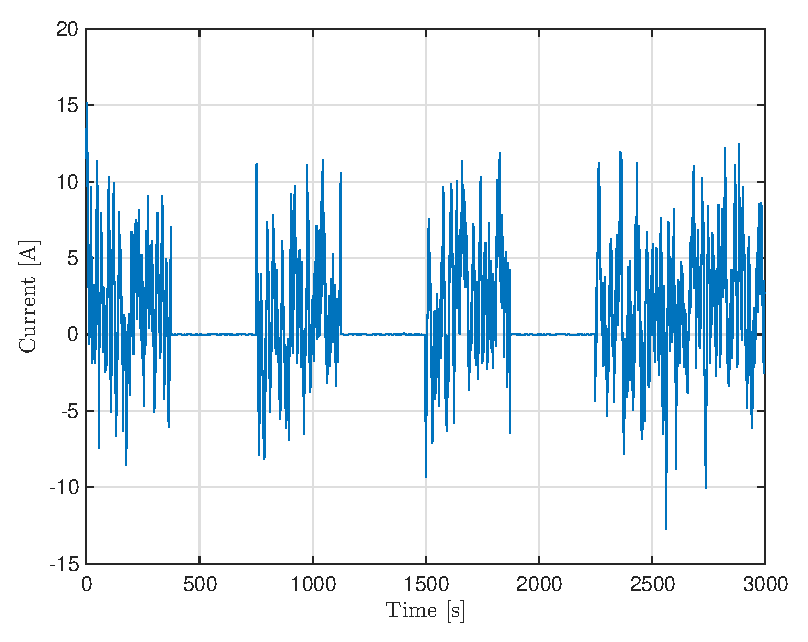
\includegraphics[width=0.5\textwidth]{figures/8/validation-I.eps}
    \caption{Current waveform used during all simulations.}
    \label{fig:8-validation-I}
\end{figure}

The same current waveform shown in Fig. \ref{fig:8-validation-I} that was recorded during the reference experiment was used for all simulations. Results of simulation with \eqref{eq:8-disc} are shown in Fig. \ref{fig:8-validation}, specifically Fig. \ref{fig:8-validation-SOC} shows the evolution of system state $SoC$ whereas Fig. \ref{fig:8-validation-U} compares the reference and simulated system output. Results confirm the expected near-perfect match of reference and simulated signals, since the reference experiment itself was a simulation, presumably using identical model parameters.

\begin{figure}[hbp]
    \centering
\begin{subfigure}{0.49\textwidth}
    \centering
    \includegraphics[width=\textwidth]{figures/8/validation-soc.eps}
    \caption{State of charge $SoC$.}
    \label{fig:8-validation-SOC}
    \end{subfigure}
    \hfill
    \begin{subfigure}{0.49\textwidth}
    \centering
    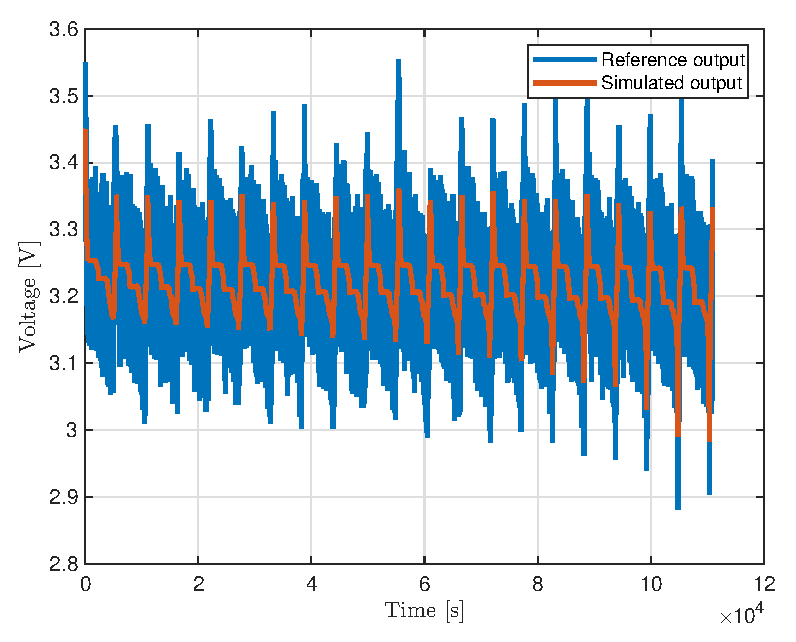
\includegraphics[width=\textwidth]{figures/8/validation-U.eps}
    \caption{Terminal voltage $\Ubat$.}
    \label{fig:8-validation-U}
    \end{subfigure}
    
    \caption{Comparison of reference and simulated waveforms.}
    \label{fig:8-validation}
\end{figure}

Assuming that the discrepancy between the simulated and reference $\Ubat$ visible in Fig. \ref{fig:8-validation-U} is purely an additive noise sequence $e$, its parameters can be extracted. The random sequence $e$ has zero mean and variance $\sigma^2 \approx 0.0013$. To assess its whiteness, its normalized autocorrelation function was evaluated and plotted in Fig. \ref{fig:8-validation-pred-error}. Since the correlation for any lag other than 0 samples is far below the 5 \% threshold, the noise sequence $e$ can be assumed white. This result is relevant for the theoretical justification of the correctness of results obtained by the Kalman Filter.


\begin{figure}[hbp]
    \centering
\begin{subfigure}{0.49\textwidth}
    \centering
    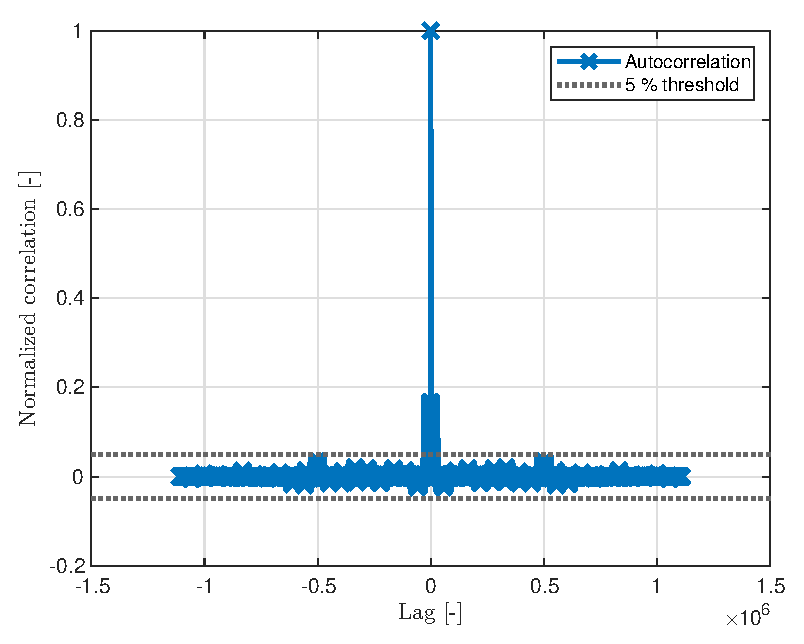
\includegraphics[width=\textwidth]{figures/8/validation-pred-error.eps}
    \caption{For all possible shifts of the signal}
    \label{fig:8-validation-pred-error-global}
    \end{subfigure}
    \hfill
    \begin{subfigure}{0.49\textwidth}
    \centering
    \includegraphics[width=\textwidth]{figures/8/validation-pred-error-detail.eps}
    \caption{Detail of the autocorrelation for low values of the signal lag}
    \label{fig:8-validation-pred-error-detail}
    \end{subfigure}
    
    \caption{Autocorrelation of the prediction error.}
    \label{fig:8-validation-pred-error}
\end{figure}

\section{EKF Implementation}

Building on top of the discrete-time model \eqref{eq:8-disc}, the Extended Kalman Filter was implemented. Apart from the state evolution and output functions, the algorithm requires their derivatives w.r.t. individual states to form time-varying Jacobian matrices
\begin{align}
    \mathbf{C}(k) &= \frac{\partial y(k)}{\partial x(k)}\biggr\rvert_{x(k),u(k)} &=& \begin{bmatrix} -1 & -1 & \frac{\partial \OCV(SoC(k))}{\partial SoC} \end{bmatrix}\biggr\rvert_{SoC(k)}, \\
        \mathbf{A}(k) &= \frac{\partial x(k+1)}{\partial x(k)}\biggr\rvert_{x(k),u(k)} = \mathbf{I} + T_s \frac{\partial f(x(k), u(k))}{\partial x(k)}\biggr\rvert_{x(k),u(k)} &=& \begin{bmatrix}
            1 - \frac{T_s}{R_1 C_1} & 0 & 0 \\ 0 & 1 - \frac{T_s}{R_2 C_2} & 0 \\ 0 & 0 & 1
        \end{bmatrix}.
\end{align}
Although the state matrix $\mathbf{A}$ is time invariant, the last element of the output matrix $\mathbf{C}(k)$ is the derivative of the cell's OCV curve that is highly dependent on the immediate $SoC(k)$. The necessity of existence of the partial derivative $\frac{\partial \OCV(SoC(k))}{\partial SoC}$ makes the lookup table implementation of the OCV curve disadvantageous and calls for a polynomial fit -- in this case approximation by a polynomial of the 5th degree shown in Fig. \ref{fig:8-ocv} together with its derivative.

\begin{figure}[H]
    \centering
    \includegraphics[width=0.5\textwidth]{figures/8/ocv_to_soc.eps}
    \caption{Polynomial approximations of the $\VOC$ curve and its derivative.}
    \label{fig:8-ocv}
\end{figure}

The single element of measurement noise covariance matrix $\mathbf{R}$ was already determined during the analysis of the additive measurement noise $e$ in Section \ref{sec:8-one} as $\mathbf{R} = \sigma^2 \approx 0.0013$. Tuning the process noise covariance matrix $\mathbf{Q}$ required several iterations and resulted in
\begin{equation}
    \mathbf{Q} = \begin{bmatrix}
    10^{-12} & 0 & 0 \\ 0 & 10^{-12} & 0 \\ 0 & 0 & 10^{-4}
\end{bmatrix}.
\end{equation}
Considering the range of reasonable values of system states and other quantities, elements of $\mathbf{Q}$ seem very small and this fact could lead to deterioration of computation accuracy. Should this ever become a problem, one could normalize system variables to obtain a more robust numerical stability. Nevertheless in this case one can easily justify matrix elements this small -- there is no reason to consider any noise apart from the additive measurement noise $e$ characterized by $\sigma^2$ that was calculated exactly using provided data. The process noise only has to cover unmodelled system dynamics. Due to symmetry, there is no reason to choose different values of variances corresponding to $U_1$ and $U_2$ and both should be far lower than the variance corresponding to $SoC$. This is because we want the EKF to primarily adjust the $SoC$ estimate to explain the observed output, whereas estimates of both polarization voltages $U_{i}$ should rely mostly on the model and should not be varied by the EKF to explain observed terminal voltages.

Results (estimates) given by the EKF are shown in Fig. \ref{fig:8-ekf}. Great gradual convergence to the true state of charge is shown in Fig. \ref{fig:8-ekf-soc}, whereas Fig. \ref{fig:8-ekf-U} shows great rejection of the additive measurement noise, as the predicted output voltage almost perfectly matches the noiseless reference output with RMSE as low as 16 mV when calculated globally and only 4 mV when calculated from $t = 2000$ onwards, where the filter has perfectly converged to the true state.

\begin{figure}[H]
    \centering
\begin{subfigure}{0.49\textwidth}
    \centering
    \includegraphics[width=\textwidth]{figures/8/ekf-soc.eps}
    \caption{State of charge $SoC$.}
    \label{fig:8-ekf-soc}
    \end{subfigure}
    \hfill
    \begin{subfigure}{0.49\textwidth}
    \centering
    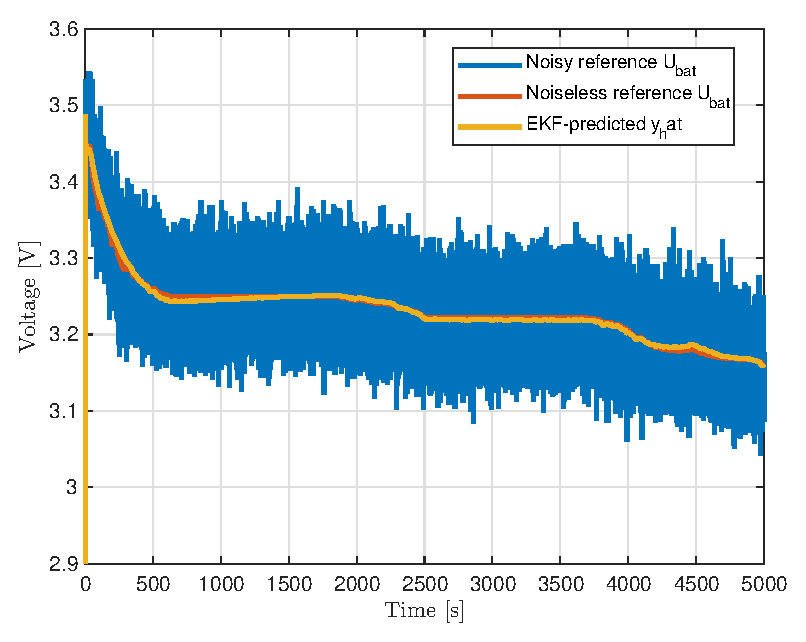
\includegraphics[width=\textwidth]{figures/8/ekf-U.eps}
    \caption{Terminal voltage $\Ubat$.}
    \label{fig:8-ekf-U}
    \end{subfigure}
    
    \caption{Comparison of reference waveforms with EKF estimates/predictions.}
    \label{fig:8-ekf}
\end{figure}

\section{Discussion}

This homework is a continuation of the previous report (HW7) that presented implementation and results for three simple methods of $SoC$ estimation. It presented many results and observations that will not be repeated, the reader is therefore advised to read its conclusions  before proceeding.

This report added a new $SoC$ estimation method based on the Extended Kalman Filter. All methods are compared in Fig \ref{fig:8-comparison} with results summarized in \ref{tab:8-comparison}. Compared to simple methods from the previous assignment, estimation by the Extended Kalman Filter enjoys a balance of robustness to the selection of initial conditions and accuracy of predicted system behavior. Observing Fig. \ref{fig:8-comparison-dev}, one may conclude that
\begin{enumerate}
    \item Even when the EKF is started with incorrect initial conditions, it eventually converges to the correct solution (unlike the Coulomb counting method), and
    \item once the EKF converges to the reference value, it never deviates far (unlike the $\OCV$ lookup method).
\end{enumerate}

\begin{figure}[hbp]
    \centering
\begin{subfigure}{0.49\textwidth}
    \centering
    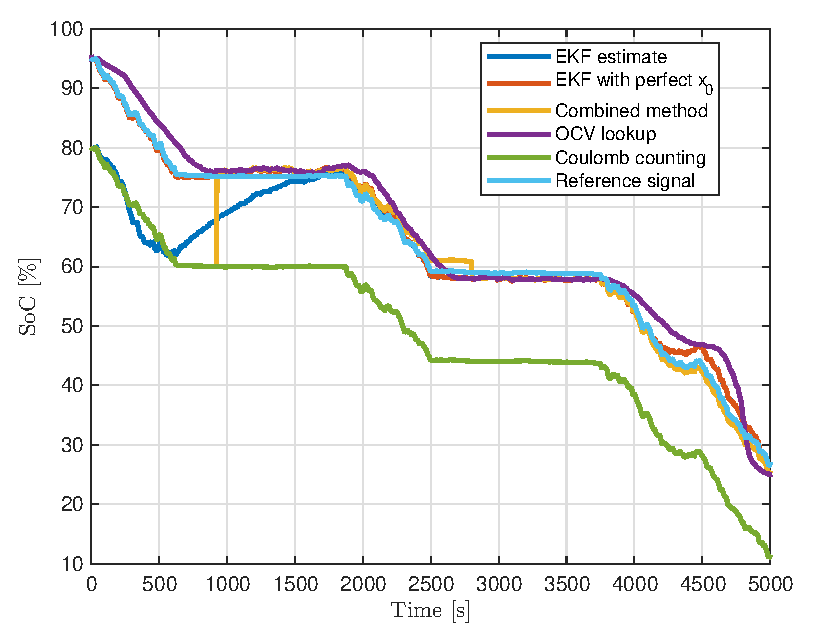
\includegraphics[width=\textwidth]{figures/8/comparison.eps}
    \caption{Absolute values of $SoC$ estimates.}
    \label{fig:8-comparison-abs}
    \end{subfigure}
    \hfill
    \begin{subfigure}{0.49\textwidth}
    \centering
    \includegraphics[width=\textwidth]{figures/8/comparison-dev.eps}
    \caption{Deviations of $SoC$ estimates from the reference.}
    \label{fig:8-comparison-dev}
    \end{subfigure}
    
    \caption{Comparison of estimation performance of individual algorithms.}
    \label{fig:8-comparison}
\end{figure}

\begin{table}[t]
    \centering
    \begin{tabular}{c|c|c}
         Method & $SoC$ RMSE [\%]& $SoC$ RMSE [\%] for $t > 2000$ s \\ \hline
         Extended Kalman Filter & 6.45 & 1.38 \\
         Coulomb Counting & 15.11 & 15.04 \\
         $\OCV$ lookup & 2.93 & 3.14 \\
         Reset-Coulomb counting & 6.62 & 1.23 \\ \hline
         Extended Kalman Filter w/ perfect ICs & 1.19 & 1.40 \\
    \end{tabular}
    \caption{Errors of estimates yielded by various methods.}
    \label{tab:8-comparison}
\end{table}

Although the OCV-lookup method achieves the lowest RMSE on the whole experiment (with the exception of EKF with perfect knowledge of initial conditions), this is caused by its ultimate lack of dynamics -- if the mean of terminal voltage $\Ubat$ was subject to more dynamical changes (e.g. due to higher current $i$), the OCV lookup estimate would quickly deteriorate as the approximated $\OCV$ would be incorrect. On the other hand, the Coulomb counting has the clear disadvantage of no correction for imprecise knowledge of initial conditions. Coulomb counting with reset solves this problem, but the correction around $t \approx \SI{900}{\second}$ is too sudden and would certainly lead to customer dissatisfaction if it happened e.g. in a smartphone or an electric vehicle. Additionally the correction performed by the reset is only as good as the OCV-lookup method, disadvantages of which were already discussed in detail in the previous report.

For these reasons, the EKF algorithm is the winner in terms of quality of the resulting estimate. One should note however that the implementation of EKF is significantly more complex and computationally demanding than any of the simpler previously discussed methods.
The EKF estimate could be further improved e.g. by using a higher-order fit of the cell's $\OCV$ curve, since the currently used model seems to deviate a little from the true waveform for $SoC < 50$ \%.





